\rhead{\small \textcolor{sugray}{Name: \hskip2.8cm}}
\rightline{\raise 10pt\hbox{\small \textcolor{sugray}%
{Midterm, 1:30--2:50\,pm, October 30, 2017}}}

\problem{10}
A poorly-trained chemical engineer named Jian
is determined to liquefy steam.
He hands you a pressure-enthalpy chart
for pure water vapor.
You notice that it is very poorly labeled.

\begin{figure}[h]\centering
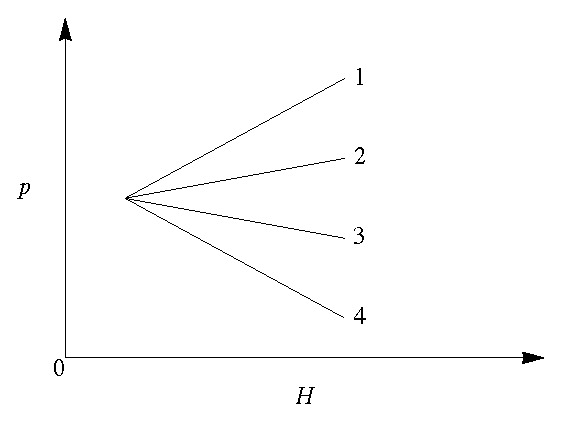
\includegraphics[width=0.3\textwidth,height=!]{pHchart}
\label{fig:pHchart}
\end{figure}
\noindent Somewhat embarrassed, he says,
``Only two curves are correct.
One has constant volume, another has constant entropy,
and both start from the same initial state.''
Using your thermodynamic expertise, determine:

\smallskip \subp Which of the two curves is correct,
and which one is which? Explain your reasoning
and clearly state any assumptions you have made.
\solution{ \\
Recall the following definitions:
\[ \dd H = \dd (U + pV) = T\,\dd S + V\,\dd p \]
\[ C_V \equiv T \pdc{S}{T}{V} \quad , \quad 
   \alpha \equiv \frac{1}{V} \pdc{V}{T}{p} \quad , \quad
   \kappa \equiv \frac{-1}{V} \pdc{V}{p}{T} \]
We need to evaluate the following partial derivatives:
\begin{align*}
    \pdc{p}{H}{V} &= \pdc{H}{p}{V}^{-1} 
  = \left[ T \pdc{S}{p}{V} + V \pdc{p}{p}{V} \right]^{-1}
  = \left[ T \pdc{S}{T}{V} \pdc{T}{p}{V} + V \right]^{-1} \\
 &= \left[ -C_V \pdc{T}{V}{p} \pdc{V}{p}{T} + V \right]^{-1}
  = \left[ \frac{-C_V (-\kappa V)}{\alpha V} + V \right]^{-1} \\
 &= \frac{1}{V + \frac{C_V \kappa}{\alpha}} \\ \\
    \pdc{p}{H}{S} &= \pdc{H}{p}{S}^{-1} = \frac{1}{V}
\end{align*}
Thermodynamic stability requires $C_V > 0$ and $\kappa > 0$. 
Assume $\alpha > 0$ - this is justified because 
our chart is for pure water vapor.
Steam expands when heated ($\alpha > 0$ for nearly all pure gases).
Applying this assumption, we know
that both curves {\bf must} have positive slope.
Additionally, since $\frac{C_V \kappa}{\alpha} > 0$, 
the constant $V$ curve has a {\bf smaller} slope than
the constant $S$ curve. 
\[ \boxed{ \text{If $\alpha > 0$ then 
           curve (1) is constant entropy
           and curve (2) is constant volume} } \]
}


\smallskip \subp If the initial volume is increased,
will the constant volume curve shift upward or downward?
\solution{\\
Thermodynamic stability requires that $\kappa > 0$,
such that pressure and volume have an inverse relationship.
Naturally, increasing the starting volume
requires a decrease in pressure, so the curve shifts down. 
This can be shown explicitly by: 
\begin{align*}
   \pdc{p}{V}{H} &= -\pdc{H}{V}{p} \pdc{p}{H}{V} 
        = -\left[ T \pdc{S}{V}{p} + V \pdc{p}{V}{p} \right] 
           \left( \frac{1}{V + \frac{C_V \kappa}{\alpha}} \right) \\
       &= -\left[ T \pdc{S}{T}{p} \pdc{T}{V}{p} + 0 \right]
           \left( \frac{1}{V + \frac{C_V \kappa}{\alpha}} \right) \\
       &= \frac{-C_p}{\alpha V} \frac{1}{V + \frac{C_V \kappa}{\alpha}} 
        = \frac{-C_p}{\alpha V^2 + \kappa C_V V} < 0
\end{align*}
Stability requires $C_p, C_v, \kappa > 0$.
Since we assumed $\alpha > 0$ above,
this expression is negative.
\[ \boxed{ \text{The curve will shift down} } \]
}


\bigskip \problem5
In class, we applied the second law to find the
most probable distribution 
for a microcanonical ensemble with $\Omega$ states. 
Specifically, we found $p_j$, the probability of observing state $j$,
by {\it extremizing} the Gibbs entropy
and {\it assuming} that it was at a maximum.
Verify this assumption - show that the $p_j$ we obtained in class
indeed corresponds to the maximum value of entropy.
\solution{\\ 
Extremizing $S = -k_B \sum_i^\Omega p_i \ln p_i$ only guarantees
that entropy is {\bf extremized}
(i.e. it could be either a minimum or maximum). 
To verify that entropy has been maximized, we need
to show that the curvature of $S$ with respect
to each $p_i$ is negative, subject to the constraint
$\sum_i^\Omega p_i = 1$.
\begin{align*}
   \frac{\dd^2}{\dd p_i^2} \left[ S - \lambda \left( 
        \sum_i^\Omega p_i - 1 \right) \right] 
&= \frac{\dd^2}{\dd p_i^2} \left[ -\kB \sum_i^\Omega p_i \ln p_i
      - \lambda \left( \sum_i^\Omega p_i - 1 \right) \right] \\
&= \frac{\dd}{\dd p_i} \left[ -\kB (\ln p_i + 1) - \lambda \right] 
 = -\frac{\kB}{p_i}
\end{align*}
In class, we showed that $p_i = \frac{1}{\Omega}$. 
Thus, the curvature is $\frac{\dd^2}{\dd p_i^2} = -\kB \Omega < 0$,
which is what we wanted to show.
\[ \boxed{ \text{Entropy is maximized because } 
           \frac{\dd^2 S}{\dd p_i^2} < 0  
           \text{ for } p_i = \frac{1}{\Omega} } \]
}

\bigskip \problem{10}
In 1973, {\sl Bekenstein} showed that
the entropy of a stationary black hole with mass $m$,
zero charge, and zero angular momentum is proportional
to the surface area of its event horizon:
\[
S = \kB \frac{c^3 A}{4 G \hbar},\quad {\rm with\ } A = 16 \pi (Gm/c^2)^2 .
\]
Here,
$\kB = \rm 1.38\times10^{-23}\, J/K$ is the Boltzmann constant,
$G = \rm 6.67\times 10^{-11}\, m^3 kg^{-1} s^{-2}$
is the gravitational constant,
$c = \rm 3.00\times 10^8\, m/s$ is the speed of light,
and $\hbar = h/(2\pi) = \rm 1.05\times 10^{-34}\, m^2 kg/s$
is the reduced Planck's constant.
The energy of a black hole is proportional to its mass,
and is given by $U = m c^2$.

\smallskip \subp
Find the temperature of a black hole
as a function of mass, $T(m)$.
\solution{\\
The first law of thermodynamics tells us that $T = \pdc{U}{S}{}$.
It doesn't matter what the other terms in $\dd U$ are 
(it doesn't matter what's held constant) because $S$
depends only on $m$ and physical constants. 
If you are curious, the other contributions to $\dd U$ 
arise from charge and angular momentum, which we have set
to a constant zero for your convenience.
\[ S = \kB \frac{c^3 A}{4 G \hbar} 
     = \frac{\kB c^3}{4 G \hbar} \frac{16 \pi G^2 m^2}{c^4} 
     = \left( \frac{4 \pi k_B G}{\hbar c} \right) m^2 \]
\begin{align*}
  T &= \pdc{U}{S}{} = \pdc{U}{m}{} \pdc{m}{S}{} 
     = \left[ \frac{\dd}{\dd m} \left( mc^2 \right) \right] 
       \left[ \frac{\dd}{\dd m} \left( 
              \frac{4 \pi k_B G}{\hbar c} m^2 \right) \right]^{-1} \\
    &= c^2 \left( \frac{\hbar c}{8 \pi k_B G m} \right) 
     = \frac{\hbar c^3}{8 \pi k_B G m}
\end{align*}
\[ \boxed{ T(m) = \frac{\hbar c^3}{8 \pi k_B G m}  
           \propto \frac{1}{m} } \]
}

\smallskip \subp
In 2015, the LIGO team detected
the merging of two black holes of masses $\rm 7.16\times 10^{31}\, kg$
and $\rm 5.77\times 10^{31}\, kg$,
which produced a new black hole of mass
$\rm 1.23\times 10^{32}\, kg$.
The leftover energy dissipated as a gravitational wave.
What is the change of entropy of the black holes alone
(ignore the gravitational wave)?
What is the temperature of the newly born black hole?
\solution{ \\
Entropy is evaluated from the provided equation:
\[ \Delta S = S_{\rm new} - S_1 - S_2 
            = \frac{4\pi \kB G}{\hbar c} 
              \left(m_{\rm new}^2 - m_1^2 - m_2^2 \right) \]
\[ \frac{4\pi \kB G}{\hbar c}  
 = \frac{4 \pi (1.38*10^{-23}\,{\rm J/K}) 
               (6.67*10^{-11}\,{\rm m^3kg^{-1}s^{-2}})}
        {(1.05*10^{-34}\,{\rm m^2kg/s}) 
         (3.00*10^8\,{\rm m/s})} 
 = 3.67*10^{-7}\,{\rm kg^{-2}~J/K} \]
\[ m_{\rm new}^2 - m_1^2 - m_2^2 
 = (1.23 * 10^{32}\,{\rm kg})^2 
 - (7.16 * 10^{31}\,{\rm kg})^2 
 - (5.77 * 10^{31}\,{\rm kg})^2 
 = 6.67*10^{63}\,{\rm kg^2} \]
\[ \boxed{ \Delta S = 2.45 * 10^{57}\,{\rm J/K} } \]
The temperature is similarly straightforward.
\[ T(m) = \frac{\hbar c^3}{8 \pi k_B G m} 
        = \frac{(1.05*10^{-34}\,{\rm m^2kg/s}) 
                (3.00*10^8\,{\rm m/s})^3}
               {8\pi (1.38*10^{-23}\,{\rm J/K}) 
                (6.67*10^{-11}\,{\rm m^3kg^{-1}s^{-2}}) 
                (1.23 * 10^{32}\,{\rm kg}) } \]
\[ \boxed{ T_{\rm new} = 9.96*10^{-10}\,{\rm K} } \]
}

\smallskip \subp
Is a black hole thermodynamically stable? Why or why not?
\solution{ \\
Stability is governed by entropy curvature.
Here, entropy is a function of only energy (mass).
\[ S = \left( \frac{4 \pi \kB G}{\hbar c} \right) m^2 \]
\[ \frac{\dd^2 S}{\dd U^2} = \frac{1}{c^4} \frac{\dd^2 S}{\dd m^2}
   = \frac{8 \pi \kB G}{\hbar c^5} > 0 \]
All the quantities in this expression are positive constants.
Since the curvature is positive, the heat capacity is negative
and the black hole is thermally unstable.
%entropy cannot be at a maximum
%(stability requires  $\frac{\dd^2 S}{\dd U^2} < 0$).
\[ \boxed{ \text{Black holes are {\bf not} thermodynamically
stable because entropy is not maximized} }\]
}

\smallskip \subp
{\bf Bonus:} The rate at which a black hole radiates energy
can be determined by treating it as a blackbody, i.e.
$ \frac{\dd U}{\dd t} = - \sigma A T^4 $.
In this equation,
$ \sigma = \rm 5.67\times 10^{-8}\, J\, m^{-2} s^{-1} K^{-4} $
is the Stefan-Boltzmann constant.
Estimate the lifetime of the newborn black hole described
in part (b).
\pts3
\solution{ \\
We would like to solve the following ODE. Note $\dd U = c^2\,\dd m$.
\[ \frac{\dd U}{\dd t} = c^2 \frac{\dd m}{\dd t} 
 = -\sigma A T^4 
 = -\sigma \left( \frac{16 \pi G^2}{c^4} m^2 \right) 
           \left( \frac{\hbar c^3}{8\pi \kB G m} \right)^4 \]
\[ \frac{\dd m}{\dd t} 
 = -\left( \frac{16 \pi \sigma G^2}{c^6} \right) 
    \left( \frac{\hbar c^3}{8\pi \kB G} \right)^4 
    \frac{1}{m^2} \]
For our own sanity, define the following lumped constants:
\[ \alpha \equiv \frac{16 \pi \sigma G^2}{c^6} 
               = 1.74*10^{-77}\,{\rm kg^{-1}s^{-1}K^{-4}} \]
\[ \beta \equiv \frac{\hbar c^3}{8\pi \kB G} 
              = 1.23*10^{23}\,{\rm kg~K}\]
The math is straightforward. Rearrange:
\[ \frac{\dd m}{\dd t} = \frac{-\alpha \beta^4}{m^2} 
   \quad \Longrightarrow \quad
   m^2 \dd m = -\alpha \beta^4 \dd t \]
\[ \int_{m_0}^{0} m^2 \dd m = -\alpha \beta^4 \int_0^\tau \dd t 
   \quad \Longrightarrow \quad 
   \frac{-m_0^3}{3} = -\alpha \beta^4 \tau \]
\[ \tau = \frac{m_0^3}{3 \alpha \beta^4} 
        = \frac{(1.23 * 10^{32}\,{\rm kg})^3}
          {3 (1.74*10^{-77}\,{\rm kg^{-1}s^{-1}K^{-4}}) 
             (1.23*10^{23}\,{\rm kg~K})^4 } 
        = 1.56*10^{80}\,{\rm s} \]
This is longer than the age of the known universe!
\[ \boxed{\tau \approx 5*10^{72}\,{\rm years} } \]
}

\bigskip \problem{15}
Denaturation of the DNA double-helix is driven by entropy.
As temperature increases, the fraction of bound base-pairs decreases.
This process can be modeled using a modified
two-state (paired/unpaired) model.
Consider a DNA double-strand $N$ bases long
at constant temperature $T$.
After applying some reasonable assumptions,
one can write its canonical partition function as:
\begin{equation}
Q(N, T) = Q_0(N, T) \left(
1 + \sigma \sum_{n=1}^{N} (N - n + 1) q^n \right),
\label{eq:Qzipper}
\end{equation}
in which $Q_0(N, T)$ is the partition function for fully denatured DNA,
$\sigma \ll 1$ is the probability of forming the first base-pair,
$n$ is an index denoting the number of consecutive paired bases, 
and $q = q(T) = e^{- \Delta E/(\kB T)}$ is
the Boltzmann factor for forming an additional base-pair,
once the first pair has been formed.

\smallskip \subp
Show that the difference in 
Helmholtz free energy between
the paired and fully-denatured states is given by 
\[
\Delta F(N, T) = - \kB T \ln\left[
1 + \frac{\sigma q \left(N(1 - q) - q(1 -q^N)\right)}{(1-q)^2}
\right] .
\]
You may find the identity $\sum_{k=1}^N r^k = \frac{r(1-r^N)}{1-r}$ helpful.
\solution{\\
Take the logarithm of $Q(N,T)/Q_0(N,T)$ to get $\Delta F(N,T)$:
\[ -\kT \ln \left( \frac{Q}{Q_0} \right) = -\kT \ln Q - \kT \ln Q_0
   = F(N,T) - F_0(N,T) = \Delta F(N,T) \]
By inspection, we need to simplify the summation in the definition of $Q(N,T)$.
\[ \sum_{n=1}^{N} (N-n+1)q^n 
 = (N+1) \sum_{n=1}^{N} q^n - \sum_{n=1}^N n q^n \]
Recall that the sum of a finite geometric series is
$\sum_{n=1}^N q^n = \frac{q(1-q^N)}{1-q}$. The first term is:
\begin{align*}
  (N+1) \sum_{n=1}^N q^n &= \frac{q(N+1)(1-q^N) }{1-q} 
      = \frac{q (N+1)(1-q^N)(1-q) }{(1-q)^2} \\
     &= \frac{(N+1)(q^{N+2}-q^{N+1}-q^2 +q)}{(1-q)^2}
\end{align*}
To get the second summation, differentiate the sum formula
to get:
\begin{align*}
    -\sum_{n=1}^N n q^n &= -\frac{q(1-(N+1)q^N + Nq^{N+1})}{(1-q)^2}
\end{align*}
Let us look at only the numerator (denominator matches goal already):
\begin{align*}
 &~ q(N+1)(q^{N+1}- q^N - q +1) - q(1-(N+1)q^N + Nq^{N+1})  \\
 &= q \left[ (N+1)(q^{N+1} - q^N - q + 1 + q^N) - 1 - N q^{N+1}  \right] \\
 &= q \left[ (N+1)(1-q) + N q^{N+1} + q^{N+1} - 1 - N q^{N+1} \right] \\
 &= q \left[ N(1-q) + 1 - q - 1 + q^N \right] \\
 &= q \left[ N(1-q) - q(1-q^N) \right]
\end{align*}
Therefore, we have shown that
\[ \frac{Q}{Q_0} = 1 + \sigma \sum_{n=1}^{N} (N-n+1)q^n 
 = 1 + \frac{\sigma q \left[ N(1-q) - q(1-q^N) \right]}{(1-q)^2} \]
\[ \boxed{ \Delta F(N,T) = - \kT \ln \left( \frac{Q}{Q_0} \right) 
 = -\kT \ln \left[ 1 + \frac{\sigma q \left( N(1-q) - q(1-q^N) \right)}
                            {(1-q)^2} \right] } \]
}

\smallskip \subp
Examine the form of the partition function in Eq.~(\ref{eq:Qzipper}).
Determine the probability of finding 
$n$ consecutive paired bases in the DNA strand,
then find an expression for the average $\ave{n}$. 
Express your final answer in terms of $N$, $\sigma$ and $q$.
\solution{\\
By inspection, each term in the summation 
is the probability weighting of the state with $n$ paired bases. 
The leading 1 corresponds to $n=0$. 
In order to convert to a true probability, we must normalize
the probability weights with $Q/Q_0$, 
which we calculated in (a).
\[ \boxed{ p_0 = \frac{1}{Q/Q_0} \qquad , \qquad 
           p_{n>0} = \frac{\sigma(N-n+1)q^n}{Q/Q_0} } \]
$\ave{n}$ can be found by using $\hat{Q} \equiv Q/Q_0$
as a generating function.
Start by using Eq. 1:
\begin{align*}
 q \pdc{\ln \hat{Q}}{q}{}
   &= 0 + \frac{q \sigma}{\hat{Q}} \sum_{n=1}^N n(N-n+1) q^{n-1} 
   = \frac{1}{\hat{Q}} \sum_{n=1}^N \sigma (N-n+1) q^{n} n \\
   &= \sum_{n=1}^N p_n n = \ave{n}
\end{align*}
Note multiplication by $q$ is necessary to get the correct weighting.
Suck it up and take the derivative using the equation from (a):
\begin{align*}
 q \pdc{\ln \hat{Q}}{q}{} &= \frac{q}{\hat{Q}} \pdc{Q}{q}{} 
   = \frac{q}{\hat{Q}} \frac{\partial}{\partial q} 
    \left[ 1 + \frac{\sigma q \left[ N(1-q) - q(1-q^N) \right]}{(1-q)^2} \right] \\
  &= \frac{\sigma q}{\hat{Q}} \left[ \frac{(1-q)^2(N(1-2q)-2q+(N+2)q^{N+1})
     + 2 q (1-q) \left[ N(1-q) - q(1-q^N) \right]} {(1-q)^4} \right] \\
  &= \frac{1}{\hat{Q}} 
     \frac{ \sigma q \left[ N(1-q)(1+q^{N+1}) - 2q(1-q^N) \right]}
          { (1-q)^3 }  \\
  &= \frac{(1-q)^2} 
          {(1-q)^2 + \sigma q \left( N(1-q) - q(1-q^N) \right) } \times
     \frac{ \sigma q \left[ N(1-q)(1+q^{N+1}) - 2q(1-q^N) \right]}
          { (1-q)^3 }  \\ 
  &= \frac{ \sigma q \left[ N(1-q)(1+q^{N+1}) - 2q(1-q^N) \right] }
          { (1-q)^3 + \sigma q (1-q) \left( N(1-q) - q(1-q^N) \right)} 
\end{align*}
The arduous journey is complete 
(there are many equivalent forms possible here):
\[ \boxed{ \ave{n} = 
   \frac{ \sigma q \left[ N(1-q)(1+q^{N+1}) - 2q(1-q^N) \right] }
        { (1-q)^3 + \sigma q (1-q) \left( N(1-q) - q(1-q^N) \right)} } \]
}

\smallskip \subp
Assuming $N$ and $\sigma$ are fixed, sketch, {\bf qualitatively},
how $\ave{n} / N$ varies with $q$ for $q$ ranging from 0 to $\infty$.
How does this trend vary with $N$?
What is the limiting behavior as $N \to \infty$, i.e.,
for extremely long DNA strands?
\solution{ \\
To get a qualitative sketch, examine limiting behavior.
Note that $0 < \frac{\ave{n}}{N} < 1$. 
When $0 \leq q \leq 1$, $\Delta E < 0$ and base-pairing
leads to an increase in energy. Qualitatively, 
we expect $\frac{\ave{n}}{N}$ to approach zero.
In the limit $q \rightarrow 0$, $(1-q) \approx 1$.
Also, we are given $\sigma \ll 1$:
\[ \lim_{q\rightarrow 0} \frac{\ave{n}}{N} \rightarrow
           \frac{1}{N}
           \frac{ \sigma q \left[ N - 2q \right] }
                { 1 + \sigma q \left( N - q \right)} 
   \approx \frac{1}{N}
           \frac{\sigma q N}{1 + \sigma q N} 
   \approx \sigma q \]
When $q < 1$, base-pairing is energetically
favorable because $\Delta E > 0$. 
We expect $\frac{\ave{n}}{N}$ will approach one.
Keep only the highest powers of $q$:
\[ \lim_{q\rightarrow \infty} \frac{\ave{n}}{N} \rightarrow
           \frac{1}{N}
           \frac{ -\sigma Nq^{N+3} + 2 \sigma q^{N+2}}
                { -\sigma q^{N+3} } 
   \approx 1 - \frac{2}{qN} \] 
Together, these two limits illustrate that the
limiting values of $\frac{\ave{n}}{N} \rightarrow 0$
and $\frac{\ave{n}}{N} \rightarrow 1$ are approached
asymptotically.
This is only possible if the curve is sigmoidal.
Examining the high $q$ limit, one can see that the first-order
correction vanishes as $N \rightarrow \infty$.
This implies that the sigmoidal approaches a step function,
and that increasing $N$ increases the `sharpness' of the curve.
The actual graph is below: \\
\begin{center}
\includegraphics[width=0.7\textwidth,height=!]{mid4c}
\end{center}
{\bf Bonus/Challenge:} Show that 
$\lim_{q \rightarrow 1} \frac{\ave{n}}{N} = \frac{1}{3}$. 
}

\smallskip \subp
In practice, the number of base-pairs in a DNA strand
is far less than infinity.
The observable average $\ave{n}$ therefore fluctuates significantly.
Write down the expression you would use to evaluate 
$\ave{(\delta n)^2}$ 
(you {\bf do not} need to simplify this expression).
\solution{ \\
Variance is typically the derivative of an expectation value.
Let's try differentiating $\ave{n}$:
\begin{align*}
    \frac{\partial \ave{n}}{\partial q} 
 &= \frac{\partial}{\partial q} 
    \left[ \frac{1}{\hat{Q}} \sum_{n=1}^N \sigma (N - n + 1) q^n n \right] \\
 &= \frac{1}{q \hat{Q}^2} \left[\hat{Q} \sum_{n=1}^N \sigma (N - n + 1) q^n n^2
  - \left( \sum_{n=1}^N \sigma (N - n + 1) q^n n \right)^2 \right] \\
 &= \frac{1}{q} \left[ \sum_{n=1}^N p_n n^2 -
                \left( \sum_{n=1}^N p_n n \right)^2 \right]
  = \frac{1}{q} \left[ \ave{n^2} - \ave{n}^2 \right]
\end{align*}
As with part (b), we need an extra factor of $q$
to get the expression we want. Thus:
\[ \boxed{ \ave{(\delta n)^2} = q \frac{\partial \ave{n}}{\partial q}
         = q \frac{\partial}{\partial q} 
           \left[ q \frac{\partial \ln (Q/Q_0)}{\partial q} \right] } \]
}

